\documentclass[oneside,a4paper,14pt]{extarticle}
\usepackage[a4paper,letterpaper,top=20mm,bottom=20mm,left=20mm,right=10mm]{geometry}
\usepackage[russian]{babel}
\usepackage{indentfirst}
\usepackage{graphicx}
\usepackage{caption}
\usepackage{titlesec}
\usepackage{minted, fancyvrb}

\titleformat{\section} {\normalsize\bfseries} {\thesection} {1em} {}
\titleformat{\subsection} {\normalsize\bfseries} {\thesubsection} {1em} {}
\titleformat{\subsubsection} {\normalsize\bfseries} {\thesubsection} {1em} {}
\renewcommand\baselinestretch{1.45}\normalsize
\setlength{\parindent}{1.25cm}

\begin{document}

\newpage
\thispagestyle{empty}
\begin{center}
	МИНИСТЕРСТВО НАУКИ И ВЫСШЕГО ОБРАЗОВАНИЯ РОССИЙСКОЙ ФЕДЕРАЦИИ ФЕДЕРАЛЬНОЕ ГОСУДАРСТВЕННОЕ БЮДЖЕТНОЕ ОБРАЗОВАТЕЛЬНОЕ УЧРЕЖДЕНИЕ ВЫСШЕГО ОБРАЗОВАНИЯ\\
	«ВЯТСКИЙ ГОСУДАРСТВЕННЫЙ УНИВЕРСИТЕТ»\\
	Институт математики и информационных систем\\
	Факультет автоматики и вычислительной техники\\
	Кафедра электронных вычислительных машин
\end{center}
\vspace{10mm}

\hfill
\begin{tabular}{l}
  \footnotesize Дата сдачи на проверку: \\
  \footnotesize <<\rule[-1mm]{5mm}{0.10mm}\/>>\rule[-1mm]{20mm}{0.10mm}\ 2025 г.\\
  \footnotesize Проверено: \\
  \footnotesize <<\rule[-1mm]{5mm}{0.10mm}\/>>\rule[-1mm]{20mm}{0.10mm}\ 2025 г. \\
\end{tabular}
\vfill

\begin{center}
    СОРТИРОВКИ ВСТАВКАМИ И ПИРАМИДАЛЬНАЯ СОРТИРОВКА: ФУНКЦИИ ПО ССЫЛКЕ И ОБРАБОТКА ФАЙЛОВ\\
	Отчёт по лабораторной работе №5\\
	по дисциплине\\
	<<Программирование>>\\
\end{center}
\vspace{25mm}
\noindent
\begin{tabular}{ll}
	Разработал студент гр. ИВТб-1301-05-00 & \rule[-1mm]{30mm}{0.10mm}\,/Черкасов А. А./   \\
	                                       & \hspace{8mm}\footnotesize(подпись)            \\
	Заместитель кафедры ЭВМ                & \rule[-1mm]{30mm}{0.10mm}\,/Долженкова М. Л./ \\
	                                       & \hspace{8mm}\footnotesize(подпись)            \\
\end{tabular}

\noindent
  \begin{tabular}{lp{58mm}r}
    Работа защищена &  & <<\rule[-1mm]{5mm}{0.10mm}\/>>\rule[-1mm]{30mm}{0.10mm}\ 2025 г.
  \end{tabular}
  \vfill

\begin{center}
	Киров\\
	2025
\end{center}

\newpage\thispagestyle{plain}

\section*{Цель}

Цель работы: Получить базовые знания о наиболее известных алгоритмах сортировки, изучить принципы работы с текстовыми файлами.

\section*{Задания}
\begin{itemize}
	\item[$-$] Реализовать сортировку данных с помощью вставок.
	\item[$-$] Реализовать сортировку данных с помощью пирамидальной сортировки.
	\item[$-$] В обоих случаях необходимо предусмотреть возможность изменения компаратора (Реализация компаратора в виде передаваемой в программу функции).
	\item[$-$] Считывание и вывод данных необходимо производить из текстового файла.
	\item[$-$] Для демонстрации работы программных реализаций самостоятельно подготовить варианты входных данных (при этом объем тестовых файлов должен позволять оценить скорость работы программ).
\end{itemize}

\section*{Решение}

Схемы алгоритмов решения задач представлена на рисунках 1 и 2. Исходный код представлен в Приложении А1.

\clearpage
\begin{figure}[H]
	\centering
	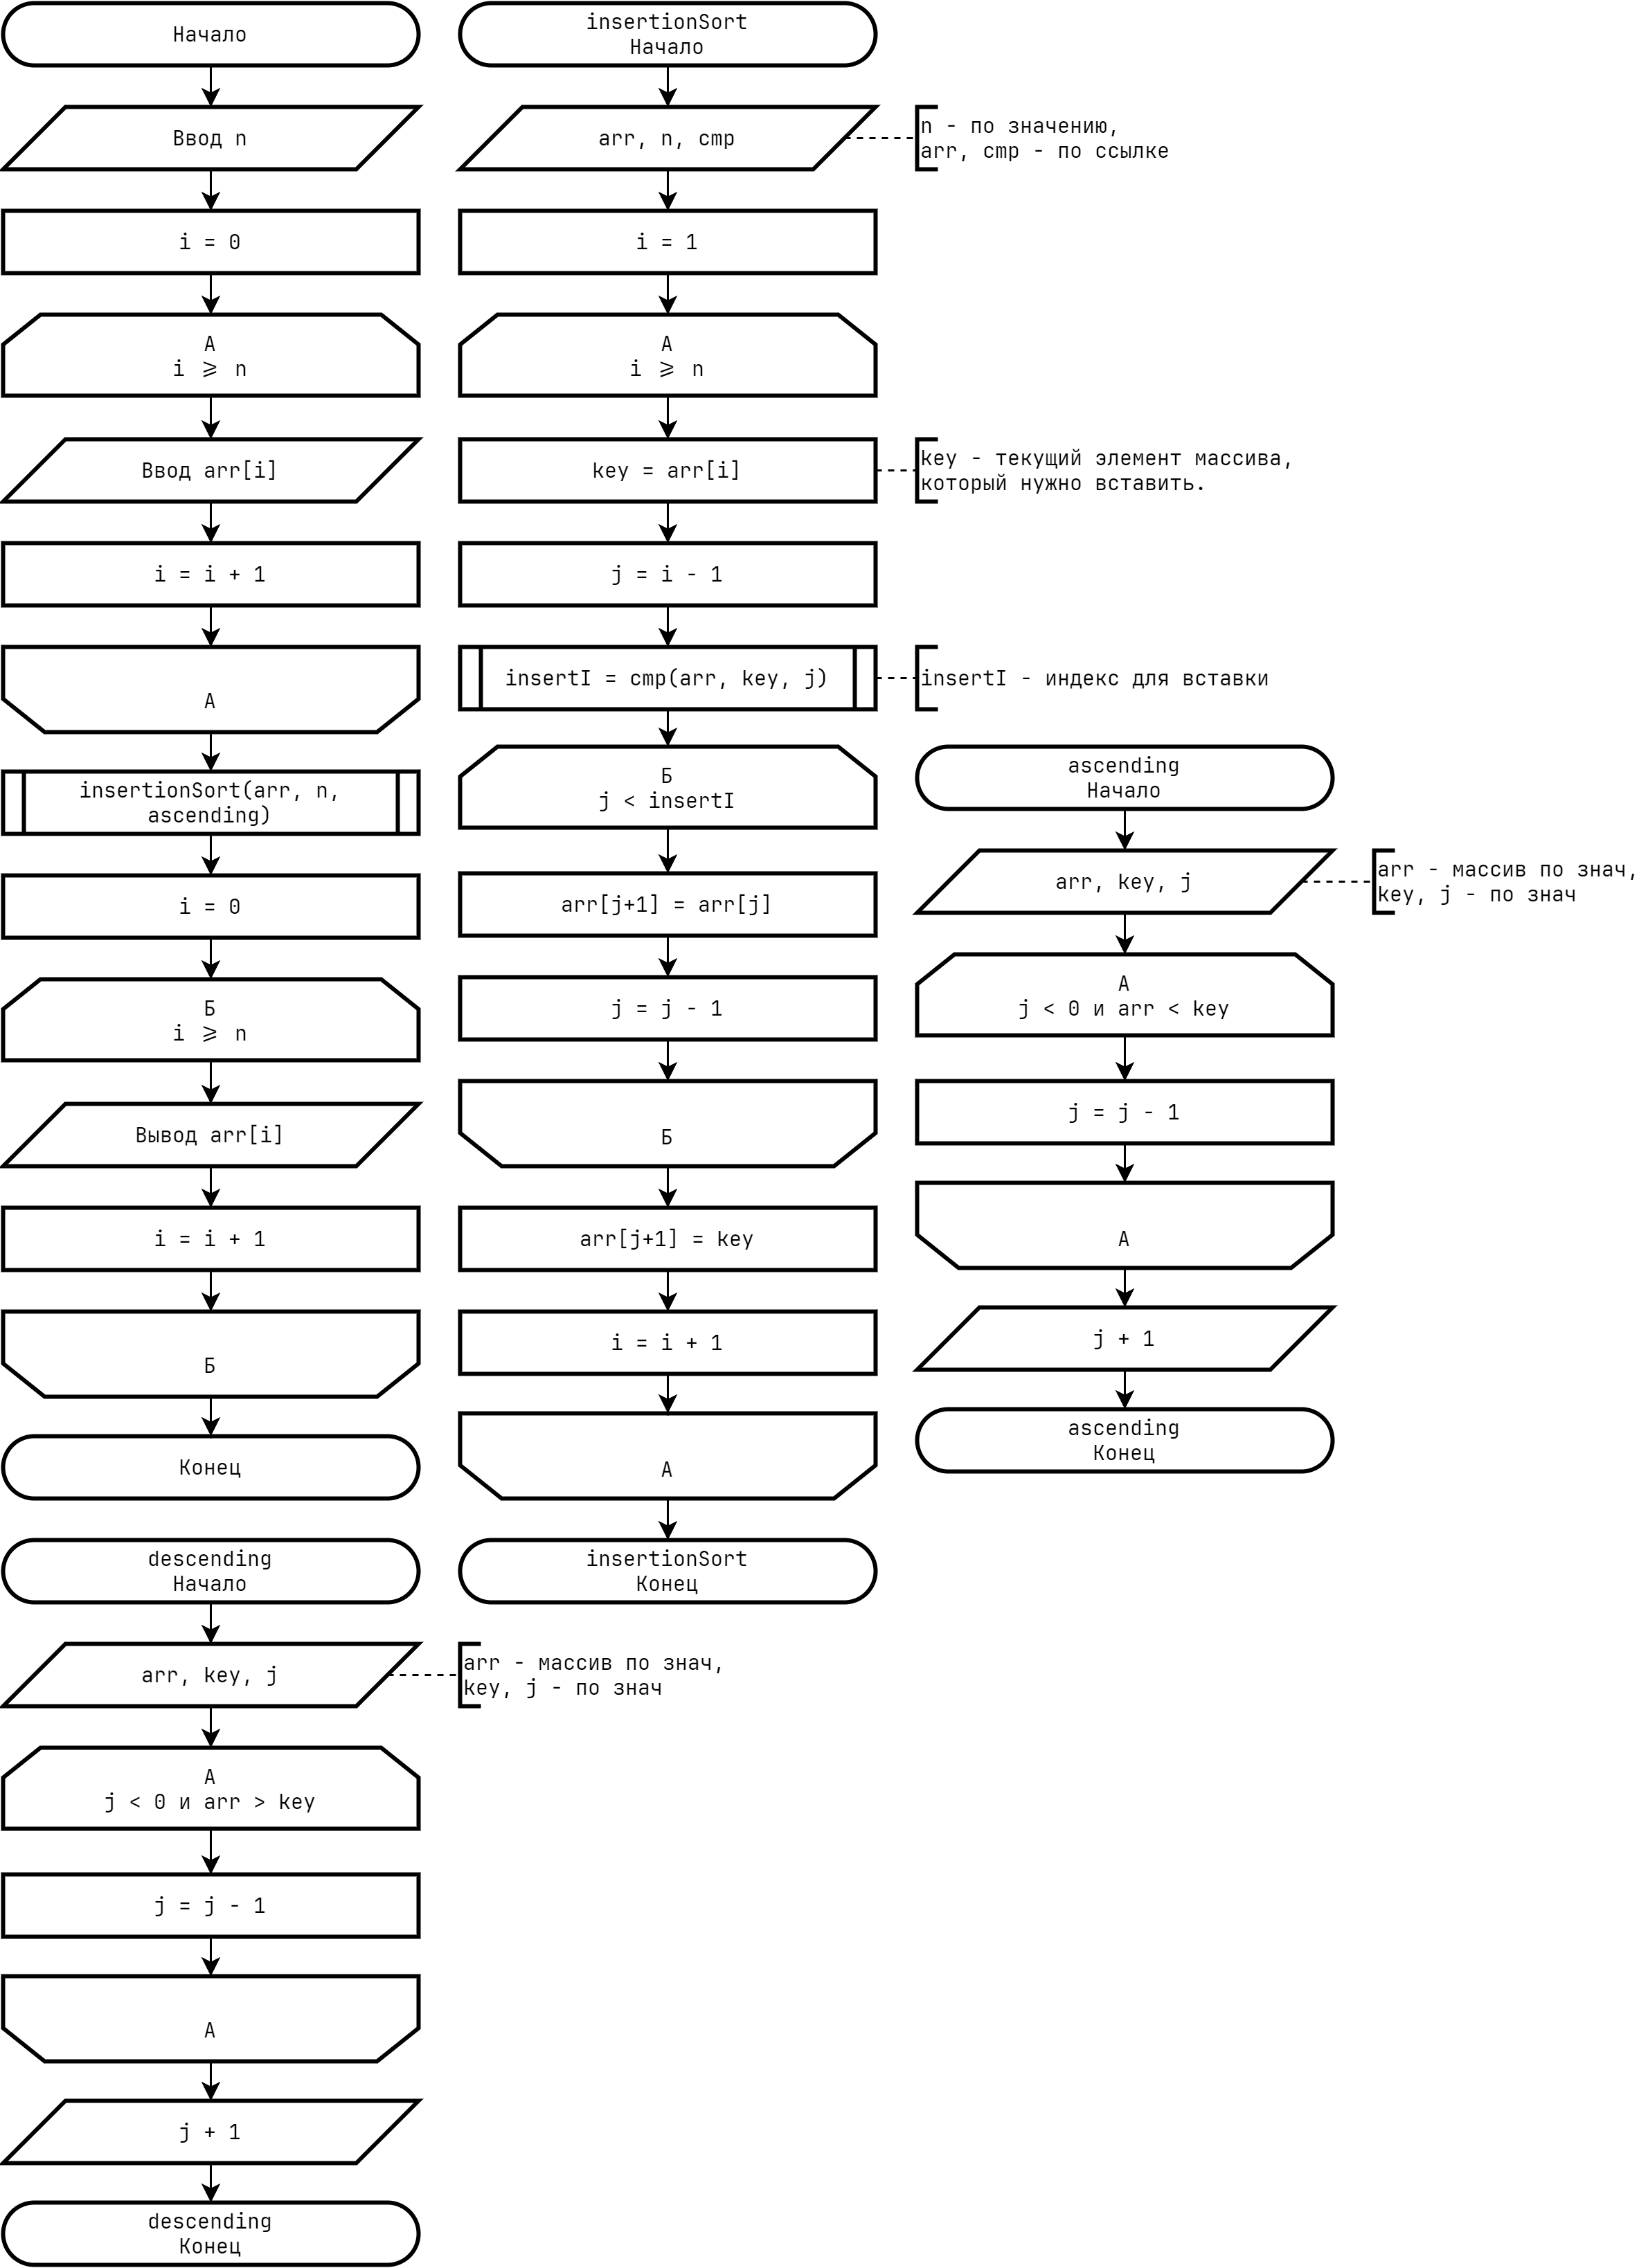
\includegraphics[height=0.9\textheight]{pics/flowchart1.png}
	\caption*{Рисунок 1 - Схема алгоритма Задания 1.}
\end{figure}

\begin{figure}[H]
	\centering
	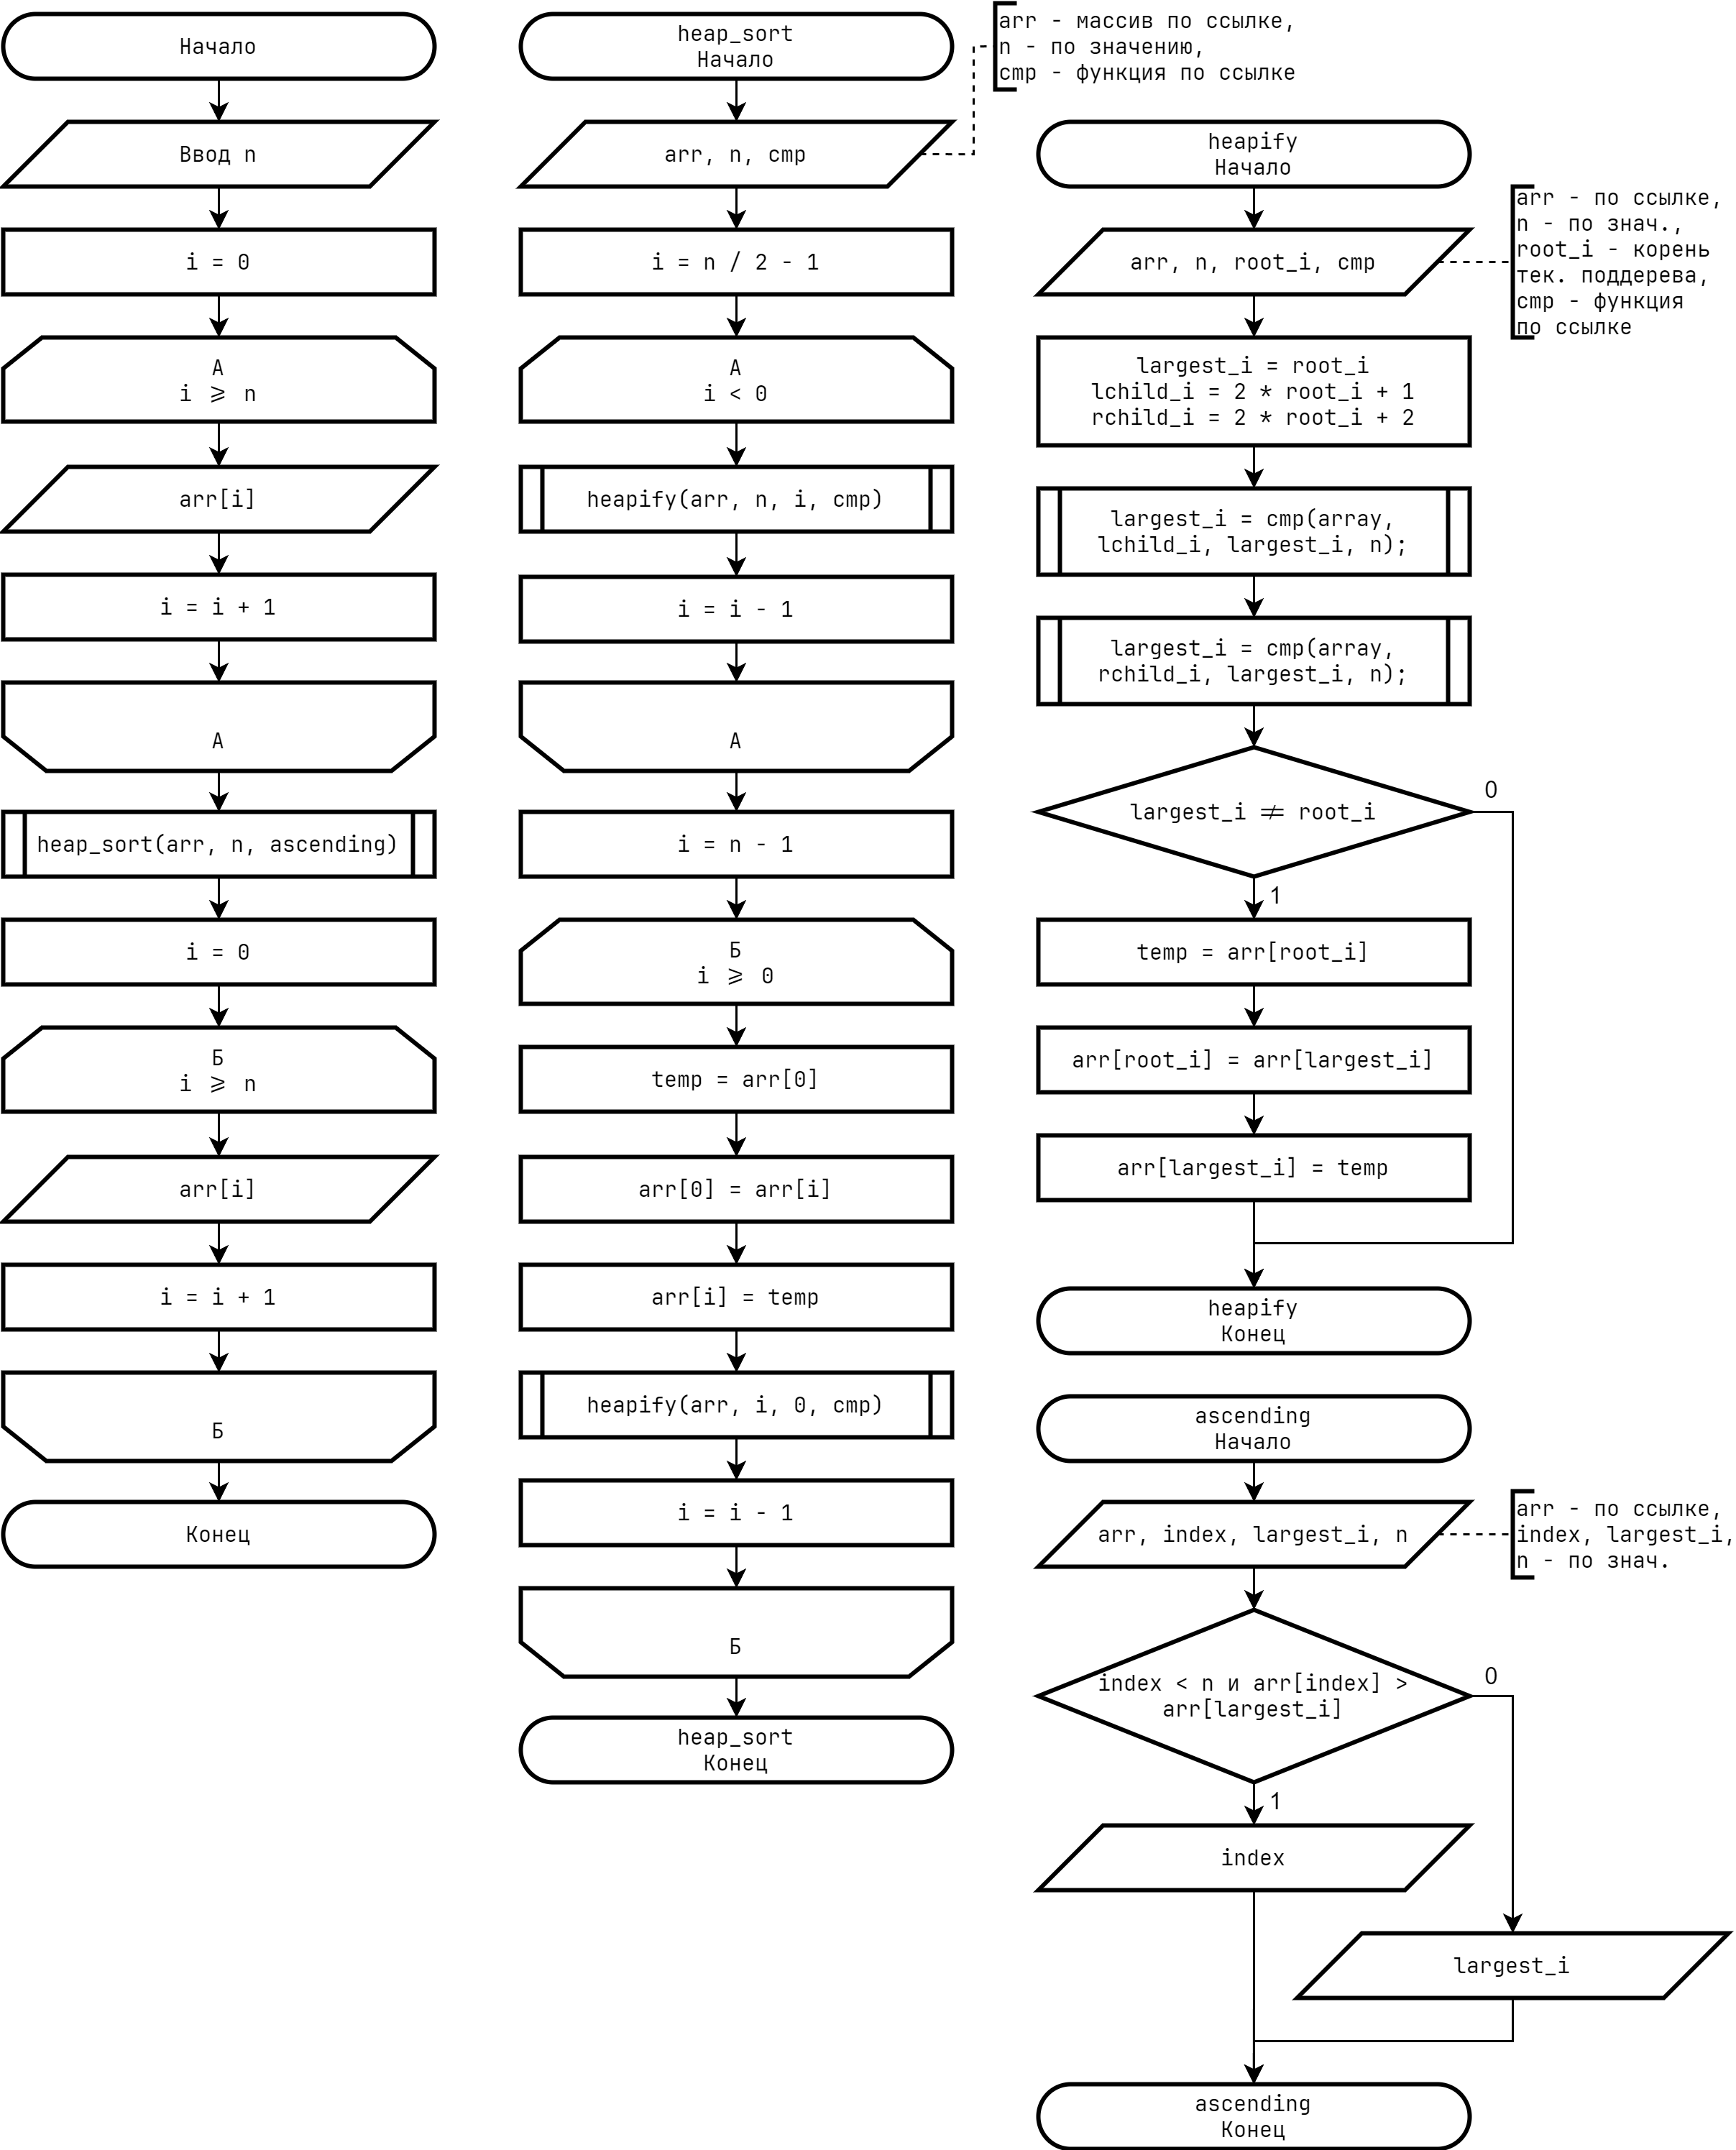
\includegraphics[height=0.9\textheight]{pics/flowchart2.png}
	\caption*{Рисунок 2 - Схема алгоритма Задания 2.}
\end{figure}

\section*{Вывод}

\setminted{style = algol, fontsize = \small} % https://pygments.org/styles/

В результате работы были реализованы алгоритмы сортировки вставками и пирамидальной сортировки с поддержкой настраиваемого компаратора и обработки текстовых файлов, что позволило оценить их эффективность и сравнить скорость работы.
\newpage
\section*{Приложение А1. Исходный код}

\inputminted{C}{code/heap_sort.c}

\section*{Приложение А2. Исходный код}
\inputminted{C}{code/insertion_sort.c}

\end{document}
